
\section{Genetic Drift and Neutral Diversity}

Various sources of randomness are inherent in evolution.  One major source of
stochasticity in population genetics is genetic drift.  Genetic drift occurs
because more or less copies of an allele by chance can be transmitted to the
next generation. This can occur because by chance the individuals carrying a
particular allele can leave more or less offspring in the next generation. In a
sexual population genetic drift also occurs because Mendelian transmission
means that only one of the two alleles in an individual, chosen at random at a
locus, is transmitted to the offspring. 

Genetic drift can play a role in the dynamics of all alleles and populations,
but it will play the biggest role for neutral alleles. A neutral polymorphism
occurs when the segregating alleles at a polymorphic site have no discernible
effect on the fitness (we'll make clear what we mean by discernible later, for
the moment think of this as ``no effect" on fitness). 


\subsection{Loss of heterozygosity due to drift.} \label{LossofHet} 

Genetic drift will, in the absence of new mutations, slowly purge our
population of neutral genetic diversity as alleles slowly drift to high or low
frequencies and are lost or fixed over time. \\

Imagine a population of a constant size $N$ diploid individuals, and that we
are examining a locus segregating for two alleles that are neutral with respect
to each other.  This population is randomly mating with respect to the alleles
at this locus. See Figures \ref{fig:LossHet_two_alleles} and
\ref{fig:LossHet_many_alleles} to see how genetic drift proceeds, by tracking
alleles within a small population. \\

In generation $t$ our current level of heterozygosity is $H_t$,
i.e. the probability that two randomly sampled alleles in generation
$t$ are non-identical is $H_t$. Assuming that the mutation rate is
zero (or vanishing small), what is our level of heterozygosity in
generation $t+1$?\\

\begin{figure}
\begin{center}
\includegraphics[width= \textwidth]{figures/Loss_of_he_col_two_alleles.png}
\end{center}
\caption{Loss of heterozygosity over time, in the absence of new
  mutations. A diploid population of 5 individuals over the
  generations, with lines showing transmission. In the first
  generation every individual is a heterozygote.} \label{fig:LossHet_two_alleles}
\end{figure} 

\begin{figure}
\begin{center}
\includegraphics[width= \textwidth]{figures/Loss_of_het_2_many_alleles.png}
\end{center}
\caption{Loss of heterozygosity over time, in the absence of new
  mutations. A diploid population of 5 individuals. In the first generation I colour every allele a different
colour so we can track their descendants.} \label{fig:LossHet_many_alleles}
\end{figure} 

In the next generation ($t+1$) we are looking at the alleles in the
offspring of generation $t$. If we randomly sample two alleles in generation
$t+1$ which had different parental alleles in generation $t$ then it
is just like drawing two random alleles from generation $t$. So the
probability that these two alleles in generation $t+1$, that have
different parental alleles in generation $t$, are non-identical is
$H_t$. \\

Conversely, if our pair of alleles have the same parental allele in
the proceeding generation (i.e. the alleles are identical by descent
one generation back) then these two alleles must be identical (as we
are not allowing for any mutation). \\

In a diploid population of size $N$ individuals there are $2N$ alleles. The
probability that our two alleles have the same parental allele in the
proceeding generation is $\nicefrac{1}{(2N)}$, the probability that they have
different parental alleles is is $1-\nicefrac{1}{(2N)}$. So by the above
argument the expected heterozygosity in generation $t+1$ is
%
\begin{equation}
H_{t+1} = \frac{1}{2N} \times 0 + \left(1-\frac{1}{2N} \right)H_t
\end{equation}
%
By this argument if the heterozygosity in generation $0$ is $H_0$ our
expected heterozygosity in generation $t$ is
%
\begin{equation}
H_t = \left(1-\frac{1}{2N} \right)^tH_0
\end{equation}
%
i.e. the expected heterozygosity with our population is decaying
geometrically with each passing generation. If we assume that $\nicefrac{1}{(2N)}
\ll 1$ then we can approximate this geometric decay by an exponential
decay (see Question \ref{geo_question} below), such that
%
\begin{equation}
H_t =H_0 \exp \left(-\frac{t}{2N} \right)  
\end{equation}
%
i.e. heterozygosity decays exponentially at a rate $\nicefrac{1}{(2N)}$.

Note how this picture of decreasing heterozygosity is in contrast to the
consistency of Hardy--Weinberg equilibrium of the previous chapter. Here, the
freqeuncy of each genotype will likely change, due to chance fluctuations in
the underlying allele frequency $p$. While within a single generation
Hardy--Weinberg proportions are maintained (at least approximately), across
generations the genotypic frequencies change with allele frequency. The change
in allele frequencies is due to drift: due to random variation in family size
and Mendelian segregation, the allele frequency in generation $t$ may differ
from that of $t+1$. We'll develop some mathematical models for these allele
frequency changes later on.

\begin{question} You are in charge of maintaining a population of delta smelt
  in the Sacramento river delta. Using a large set of microsatellites you
  estimate that the mean level of heterozygosity in this population is 0.005.
  You set yourself a goal of maintaining a level of heterozygosity of at least
  0.0049 for the next two hundred years. Assuming that the smelt have a
  generation time of 3 years, and that only genetic drift affects these loci.
  What is the smallest fully outbreeding population that you would need to
maintain to meet this goal?  (Note that while these numbers are made up, this
is similar to the calculations being carried out by conservation biologists).
\end{question}

\begin{question} \label{geo_question} In mathematical population genetics, a
  commonly used approximation $(1-x) \approx e^{-x}$ for $x << 1$ (formally
  this follows from the Taylor series expansion of $\exp(-x)$ ignoring second
  order terms of $x$).  This is especially useful for approximating a geometric
  decay process by an exponential decay process, e.g. $(1 - x)^t \approx
  e^{-xt}$. Using R, check how good of an approximation this is for three
  values of x, $x = 0.5, 0.1, 0.01$. Do this by plotting the geometric decay as
  points, and the exponential decay as a curve, using different colors for each
  of these three values. Note that you should have a discrete timescale for the
  geometric decay (e.g. using \texttt{seq(0, 18)}) and a near continuous scale
  for the exponential decay (e.g. using \texttt{seq(0, 18, length.out=100)}.
  Print off some of your graphs and hand them in. 

    % max <- 18; x <- seq(0, max); x1 <- seq(0, max, length.out=100); plot(x, (1-0.5)^x, col='purple', pch=19); lines(x1, exp(-0.5*x1), col='purple'); points(x, (1-0.1)^x, pch=19, col='orange'); lines(x1, exp(-0.1*x1), col='orange'); points(x, (1-0.01)^x, pch=19, col='green'); lines(x1, exp(-0.01*x1), col='green') # messy but works

\end{question}

\subsection{Levels of diversity maintained by a balance between
 mutation and drift} \label{DriftMutationBalance}

Looking backwards in time from one generation to the next, we are going to say
that two alleles which have the same parental allele (i.e. find their common
ancestor) in the preceding generation have \emph{coalesced}, and refer to this
event as a \emph{coalescent event}.

The probability that our pair of randomly sampled alleles have coalesced in the
preceding generation is $\nicefrac{1}{(2N)}$, the probability that our pair of
alleles fail to coalesce is $1-\nicefrac{1}{(2N)}$. 

The probability that a mutation changes the identity of the
transmitted allele is $\mu$ per generation. So the probability of no
mutation occurring is $(1-\mu)$. We'll assume that when a mutation
occurs it creates some new allelic type which is not present in the
population. This assumption (commonly called the infinitely-many-alleles model) makes the math slightly cleaner, and also
is not too bad an assumption biologically. See Figure
\ref{fig:Mut_Sel_balance} for a depiction of mutation-drift balance in
this model over the generations.

This model let's us calculate when our two alleles last shared a common
ancestor and whether these alleles are identical as a result of
failing to mutate since this shared ancestor.  For example we can work out the probability that our
two randomly sampled alleles coalesced $2$ generations in the past
(i.e. they fail to coalesce in generation $1$ and then coalescent in
generation $2$), and
that they are identical as
\begin{equation}
\left(1- \frac{1}{2N} \right) \frac{1}{2N} (1-\mu)^4
\end{equation}
note the power of $4$ is because our two alleles have to have failed
to mutate through $2$ meioses each.

More generally the probability that our alleles coalesce in generation
$t+1$ and are identical due to no mutation to either allele in the
subsequent generations is
%
\begin{equation}
P(\textrm{coal. in t+1 \& no mutations}) =  \frac{1}{2N} \left(1- \frac{1}{2N} \right)^t \left(1-\mu \right)^{2(t+1)}
\end{equation}
%
to make this slightly easier on ourselves let's further assume that $t
\approx t+1$ and so rewrite this as:
\begin{equation}
P(\textrm{coal. in t+1 \& no mutations}) \approx \frac{1}{2N} \left(1- \frac{1}{2N} \right)^t \left(1-\mu \right)^{2t}
\end{equation}
%

This gives us the approximate probability that two alleles will coalesce in the
$(t+1)^\text{th}$ generation. In general, we may not know when two alleles may
coalesce: they could coalesce in generation $t=1, t=2, \ldots $, and so on.
Thus, to calculate the probability that two alleles coalesce in \emph{any}
generation before mutating, we can write:

\begin{align*}
  P(\textrm{coal. in any generation \& no mutations}) &\approx P(\textrm{coal. in} \; t=1 \; \textrm{\& no mutations}) \; + \\ 
&  P(\textrm{coal. in} \; t=2 \; \textrm{\& no mutations}) + \ldots \\
  %P(\textrm{coal. in} \; t=3 \; \textrm{\& no mutations})  +\ldots \\
  &= \sum_{t=1}^\infty P(\textrm{coal. in } \; t \; \textrm{generations \& no mutation})
\end{align*}
%
which follows from the fact that coalescing in a particular generation is
mutually exclusive with coalescing in a different generation and basic probability.

While we could calculate a value for this sum given $N$ and $\mu$, it's
difficult to get a sense of what's going on with such a complicated expression.
Here, we turn to a common approximation in population genetics (and all applied
mathematics), where we assume that $\nicefrac{1}{(2N)} \ll 1$ and $\mu \ll 1$.
This allows us to approximate the geometric decay as an exponential decay.
Then, the probability two alleles coalesce in generation $t+1$ and don't mutate
can be written as:
%
\begin{align} P(\textrm{coal. in t+1 \& no mutations}) &\approx \frac{1}{2N}
\left(1- \frac{1}{2N} \right)^t \left(1-\mu \right)^{2t} \\ 
& \approx \frac{1}{2N} e^{-t/(2N)} e^{-2\mu t } \\
&=\frac{1}{2N} e^{-t(2\mu+1/(2N))} \end{align} 
%
and then we simply approximate the summation by an integral, giving us:
%
\begin{figure} \begin{center} \includegraphics[width= 0.8
\textwidth]{figures/Mut_drift_balance.png} \end{center} \caption{Mutation-drift
balance. A diploid population of 5 individuals. In the first generation
everyone has the same allele (black). Each generation the transmitted allele
can mutate and we generate a new colour. In the bottom plot I trace the
frequency of alleles in our population over time.} \label{fig:Mut_Sel_balance}
\end{figure} 

\begin{equation}
\frac{1}{2N} \int_0^{\infty} e^{-t(2\mu+1/(2N))} dt =
\frac{1/(2N)}{1/(2N)+2\mu} = \frac{1}{1+4N\mu}
\end{equation}

Doing so gives us the probability that our two alleles coalesce at some point
in time, and do not mutate on either ancestral lineage to their common
ancestor. Equivalently, this can be thought about as the probability our two
alleles coalesce \emph{before} mutating.

Then, the complementary probability that our pair of alleles are non-identical
(or heterozygous) is simply one minus this, i.e.
\begin{equation}
\frac{4N\mu}{1+4N\mu} \label{eqn:hetero}
\end{equation}
This compound parameter $4N\mu$, the population-scaled mutation rate,
will come up a number of times so we'll give it its own name
\begin{equation}
\theta = 4N\mu
\end{equation}

So all else being equal, species with larger population sizes should
have proportionally higher levels of neutral polymorphism. 

\subsection{The effective population size}
In practice populations rarely conform to our assumptions of being
constant in size with low variance in reproduction success. Real
populations experience dramatic fluctuations in size, and there is
often high variance in reproductive success. Thus rates of drift in
natural populations are often a lot higher than the census population
size would imply.\\

To cope with this population geneticists often invoke the concept of
an effective population size ($N_e$). In many situations (but not all), departures from model assumptions can be captured by substituting $N_e$ for $N$.

Specifically the effective population size ($N_e$) is the population size that
would result in the same rate of drift in an idealized constant population size
as that observed in our true population (following our modeling assumptions).
\\

If population sizes vary rapidly in size, we can (if certain conditions are met)
replace our population size by the harmonic mean population size.
Consider a diploid population of variable size, whose size is $N_t$ $t$ generations into the
past. The probability our pairs of alleles have not coalesced by the generation $t^{th}$ is
given by
\begin{equation}
\prod_{i=1}^{t} \left(1-\frac{1}{2N_t} \right)
\end{equation}
note that this is simply collapses to our original expression
$\left(1-\frac{1}{2N } \right)^t $ if $N_i$ is constant. If $1/(N_i)$ is
small, then we can approximate $1-\frac{1}{2N_i}$ by
$\exp(-\frac{1}{2N_i})$. Such that if $N_i$ is never too small
\begin{equation}
\prod_{i=1}^{t} \left(1-\frac{1}{2N_i} \right)
\approx \prod_{i=1}^{t} \exp \left( -\frac{1}{2N_i} \right)   =
\exp \left(- \sum_{i=1}^{t} \frac{1}{2N_i} \right) .
\end{equation}
In our constant population size case
the probability of failing to coalesce is $\exp(-t/(2N))$. So the
variable population coalescent probabilities are still of the same form but
the exponent has changed. Comparing the exponent in the two cases we see
\begin{equation}
\frac{t}{2N} = \sum_{i=1}^{t} \frac{1}{2N_i}
\end{equation}
so that if we want a constant effective population size ($N_e$) that has the same
coalescent probability as our variable population we need to set
$N=N_e$ and rearrange this to see
\begin{equation}
N_e =\frac{1}{\frac{1}{t} \sum_{i=1}^{t} \frac{1}{N_i} }.
\end{equation}
this is the harmonic mean of the varying population size. Thus our
effective population size, the size of an idealized constant
population which matches the rate of genetic drift, is the harmonic
mean true population size over time. The harmonic mean is very
strongly affected by small values, such that if our population size is
one million $99\%$ of the time but drops to a $1000$ every hundred or
so generations, $N_e$ will be much closer to $1000$ than a
million. See Figure \ref{fig:LossHet_varying_pop}  for a depiction of
a repeatedly bottlenecked population losing diversity at a fast rate.\\

\begin{figure}
\begin{center}
\includegraphics[width= \textwidth]{figures/Loss_of_he_col_alleles_varying_pop_dark.png}
\end{center}
\caption{Loss of heterozygosity over time in a bottlenecking population. A diploid population of 10 individuals, that bottlenecks
  down to three individuals repeatedly. In the first generation I colour every allele a different
colour so we can track their descendants, there are no new
  mutations.} \label{fig:LossHet_varying_pop}  
\end{figure} 

%would result in the same rate of drift
%Luckily, in many (not all) situations, departures from model assumptions can be captured by substituting Ne for N, i.e., by plugging in a fictitious N that leads to the same level of genetic drift as observed.

Variance in reproductive success will also affect our effective
population size. Even if our population has a large constant size of $N$
individuals, if only small proportion of them get to reproduce then
the rate of drift will reflect this much small number of reproducing
individuals. See Figure \ref{fig:LossHet_varying_RS} for a depiction of the higher rate of drift
in a population where there is high variance in reproductive success.

 If only $N_M$ males get to contribute to the next
generation and $N_F$ females get to contribute to the next
generation. When our two alleles pick an ancestor, $25\%$ of the time
our alleles were both in a female ancestor in which case they coalesce
with probability $1/(2N_F)$, and $25\%$ of the time they are both in a
male ancestor in which case they coalesce with probability
$1/(2N_M)$. The remaining $50\%$ of the time our ancestral lineages
are in two individuals are different sexes in a generation so cannot
coalescence.  Therefore, our probability of coalescence in the preceding
generation is
\begin{equation}
\frac{1}{4}\frac{1}{2N_M}+\frac{1}{4}\frac{1}{2N_F} =
\frac{1}{8}\frac{N_F+N_M}{N_FN_M} 
\end{equation}
i.e. the rate of coalescence is the harmonic mean of the two
sexes population sizes, 
equating this to $\frac{1}{2N_e}$ we find
\begin{equation}
N_e = \frac{4N_FN_M}{N_F+N_M}
\end{equation}
Thus if reproductive success is very skewed in one sex (e.g. $N_M \ll
N/2$) our effective population size will be much reduced as a result.\\


\begin{figure}
\begin{center}
\includegraphics[width= \textwidth]{figures/Loss_of_he_col_alleles_varying_RS.png}

\end{center}
\caption{High variance on reproductive success increases the rate of genetic drift. A diploid population of 10 individuals, where the circled
  individuals have much higher reproductive success. In the first generation I colour every allele a different
colour so we can track their descendants, there are no new
  mutations.} \label{fig:LossHet_varying_RS}
\end{figure} 


\subsection{The Coalescent and patterns of neutral diversity}

\paragraph{Pairwise Coalescent time distribution and the number of
 pairwise differences.}
Thinking back to our calculations we made about the loss of neutral heterozygosity
and equilibrium levels of diversity (in Sections \ref{LossofHet} and \ref{DriftMutationBalance}), you'll note that we could first specify
what generation a pair of sequences coalesce in, and then calculate
some properties of heterozygosity based on that. That's because neutral
mutations do not affect the probability that an individual transmits
that allele, so don't affect the way in which we can trace ancestral lineages
back. \\

As such it will often be helpful to consider the time to the common
ancestor of a pair of sequences, and then think of the impact of that
on patterns of diversity. See Figure \ref{fig:Coalescent_simulation}
for an example of this. The probability that a pair of alleles
have failed to coalesce in $t$ generations and then coalesce in the
$t+1$ generation back is
\begin{equation}
  \frac{1}{2N} \left(1- \frac{1}{2N} \right)^{t} \approx \frac{1}{2N} e^{-t/(2N)} \label{eqn:coal_time_dist}
\end{equation}
thus the coalescent time of a pair of sequences ($T_2$) is
approximately exponentially distributed with a rate $1/(2N)$. We'll denote that by
saying that $T_2 \sim \text{Exp}\left( 1/(2N) \right)$. The mean coalescent
time of a pair of a pair of alleles is $2N$ generations\\


\begin{figure}
\begin{center}
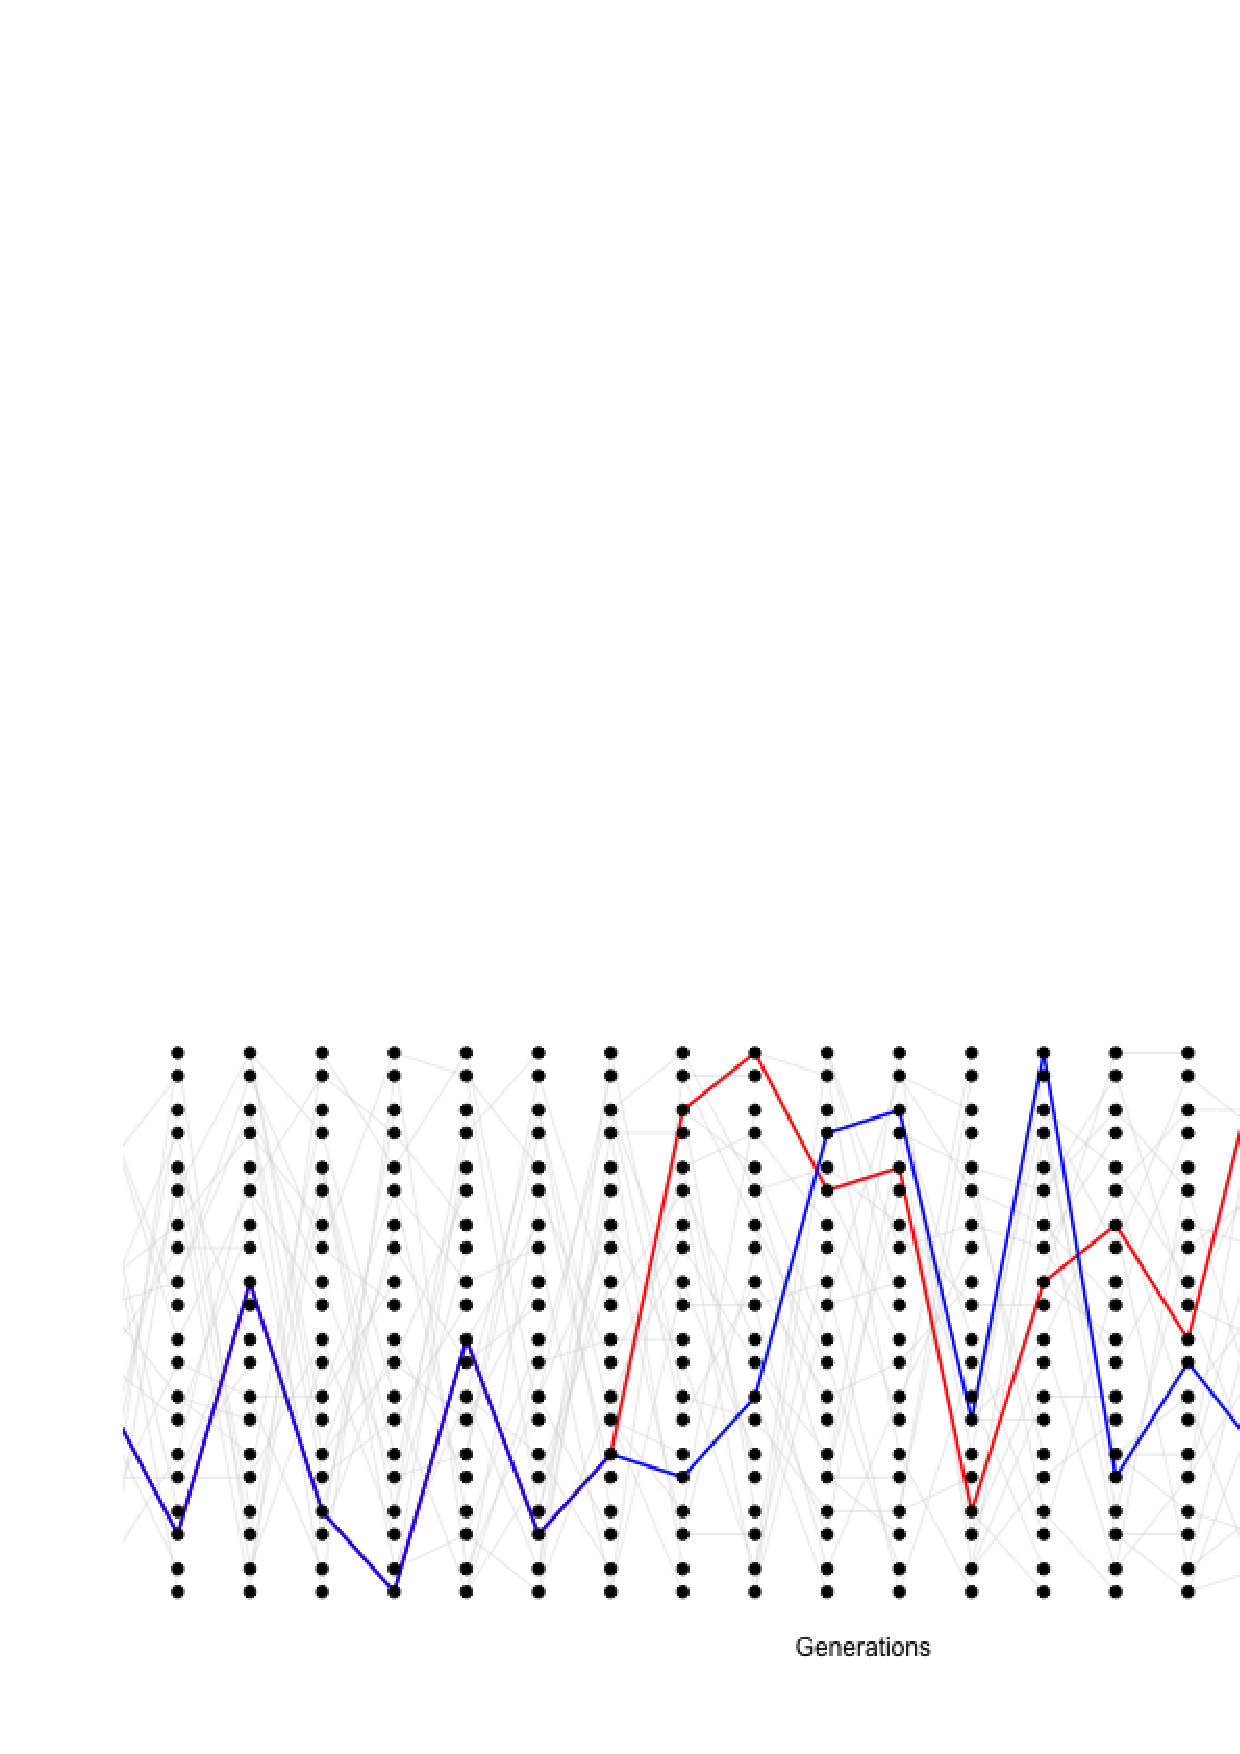
\includegraphics[width=\textwidth]{figures/Coalescent.png}
\end{center}
\caption{A simple simulation of the coalescent process. The simulation
  consists of a diploid population of 10 individuals (20 alleles). In
  each generation, each individual is equally likely to be the parent
  of an offspring (and the allele transmitted is indicated by a light
  grey line).  We track a
  pair of alleles, chosen in the present day, back 14 generations
  untill they find a common ancestor.} \label{fig:Coalescent_simulation}
\end{figure}



Conditional on a pair of alleles coalescing $t$ generations ago
there are $2t$ generations in which a mutation could occur. Thus the
probability of our pair of alleles are separated by $j$ mutations
since they last shared a common ancestor is
\begin{equation}
P(j | T_2 = t ) = {2t \choose j} \mu^{j} (1-\mu)^{2t-j}
\end{equation}
i.e. mutations happen in $j$ generations, and do not happen in $2t-j$
generations (with ${2t \choose j}$ ways this can possibly
happen). Assuming that $\mu \ll 1$, and that $2t-j \approx 2t$ then we
can approximate the probability that we have $j$ mutations as a
Poisson distribution
\begin{equation}
P(j | T_2 = t ) = \frac{ (2 \mu t )^{j} e^{-2\mu t}}{j!}
\end{equation}
i.e. a Poisson with mean $2\mu t $. \\

As our expected coalescent time is $2N$ generations (which follows from the expected value of exponential distributions), the expected
number of mutations separating two alleles drawn at random from the
population is
%
\begin{align}
  \E(j) &= 2\mu\E(t) \\ \nonumber
  &= 4N\mu \\
  &= \theta \nonumber
\end{align}
We'll assume that mutations never happen at the same site twice,
i.e. no multiple hits, such that we get to see all of the mutation events that separate our pair
of sequences (we'll call this the infinitely-many-sites assumption,
which should be fine if $N\mu_{BP} \ll 1$, where $\mu_{BP}$ is the mutation rate per base pair). Thus the number of
mutations between a pair of sites is the observed number of
differences between a pair of sequences. \\

We'll denote the observed number of pairwise differences at putatively neutral
sites separating a pair of sequences as $\pi$ (we usually average this over a
number of pairs of sequences for a region). So we can estimate of $\theta$ from
$\pi$, $\widehat{\theta}_{\pi}$ by setting $\widehat{\theta}_{\pi}=\pi$.  If we
have an independent estimate of $\mu$, then from setting $\pi =
\widehat{\theta}_{\pi} = 4N\mu$ we can obtain an estimate of the population
size $N$ that is consistent with our levels of neutral polymorphism.

\begin{question}
Robinson et al. (Current Biology 2016) report $\pi$ for sample from
populations of the California mainland gray fox and
the San Nicolas Channel Island fox to be 0.0012 and 0.000014
respectively. \\
{\bf A)} How many sites do you expect to differ between two samples
sequenced over a 100kb region in each of these populations?\\   
{\bf B)} Assuming a mutation rate of $2\times 10^{-8}$ what
effective population size do you estimate for these two populations?
\\
{\bf C)} Why is the effective population size of the Channel Island fox
so low? [Hint: quickly google Channel island foxes to read up on their
history, also to see how ridiculously cute they are.]
\end{question}

\subsection{The coalescent process of a sample of alleles.}

Usually we are not just interested pairs of alleles, or the
average pairwise diversity, we are interested in the properties of
diversity in samples of a number of alleles drawn from the population.  
To allow for this instead of just following a pair of lineages back until they
coalesce, we can follow the history of a sample of alleles back
through the population.

Consider first sampling three alleles at random from the population. The
probability that all three alleles choose exactly the same ancestral allele one
generation back is $\nicefrac{1}{(2N)^2}$. If $N$ is reasonably large then this
is a very small probability. As such it is very unlikely that our three alleles
coalesce at once, a in a moment we'll see that it is safe to ignore such
unlikely events. \\

The probability that a specific pair of alleles find a common ancestor in the
preceding generation is still $\nicefrac{1}{(2N)}$. There are three possible pairs of
alleles so the probability that no pair finds a common ancestor is
\begin{equation}
\left(1-\frac{1}{2N} \right)^3 \approx \left( 1- \frac{3}{2N} \right)
\end{equation}
in making this approximation we are multiplying out the right hand-side
and ignoring terms of $1/N^2$ and higher. See
Figure \ref{fig:Coalescent_simulation_3} for a random realization of this process. \\


\begin{figure}
\begin{center}
  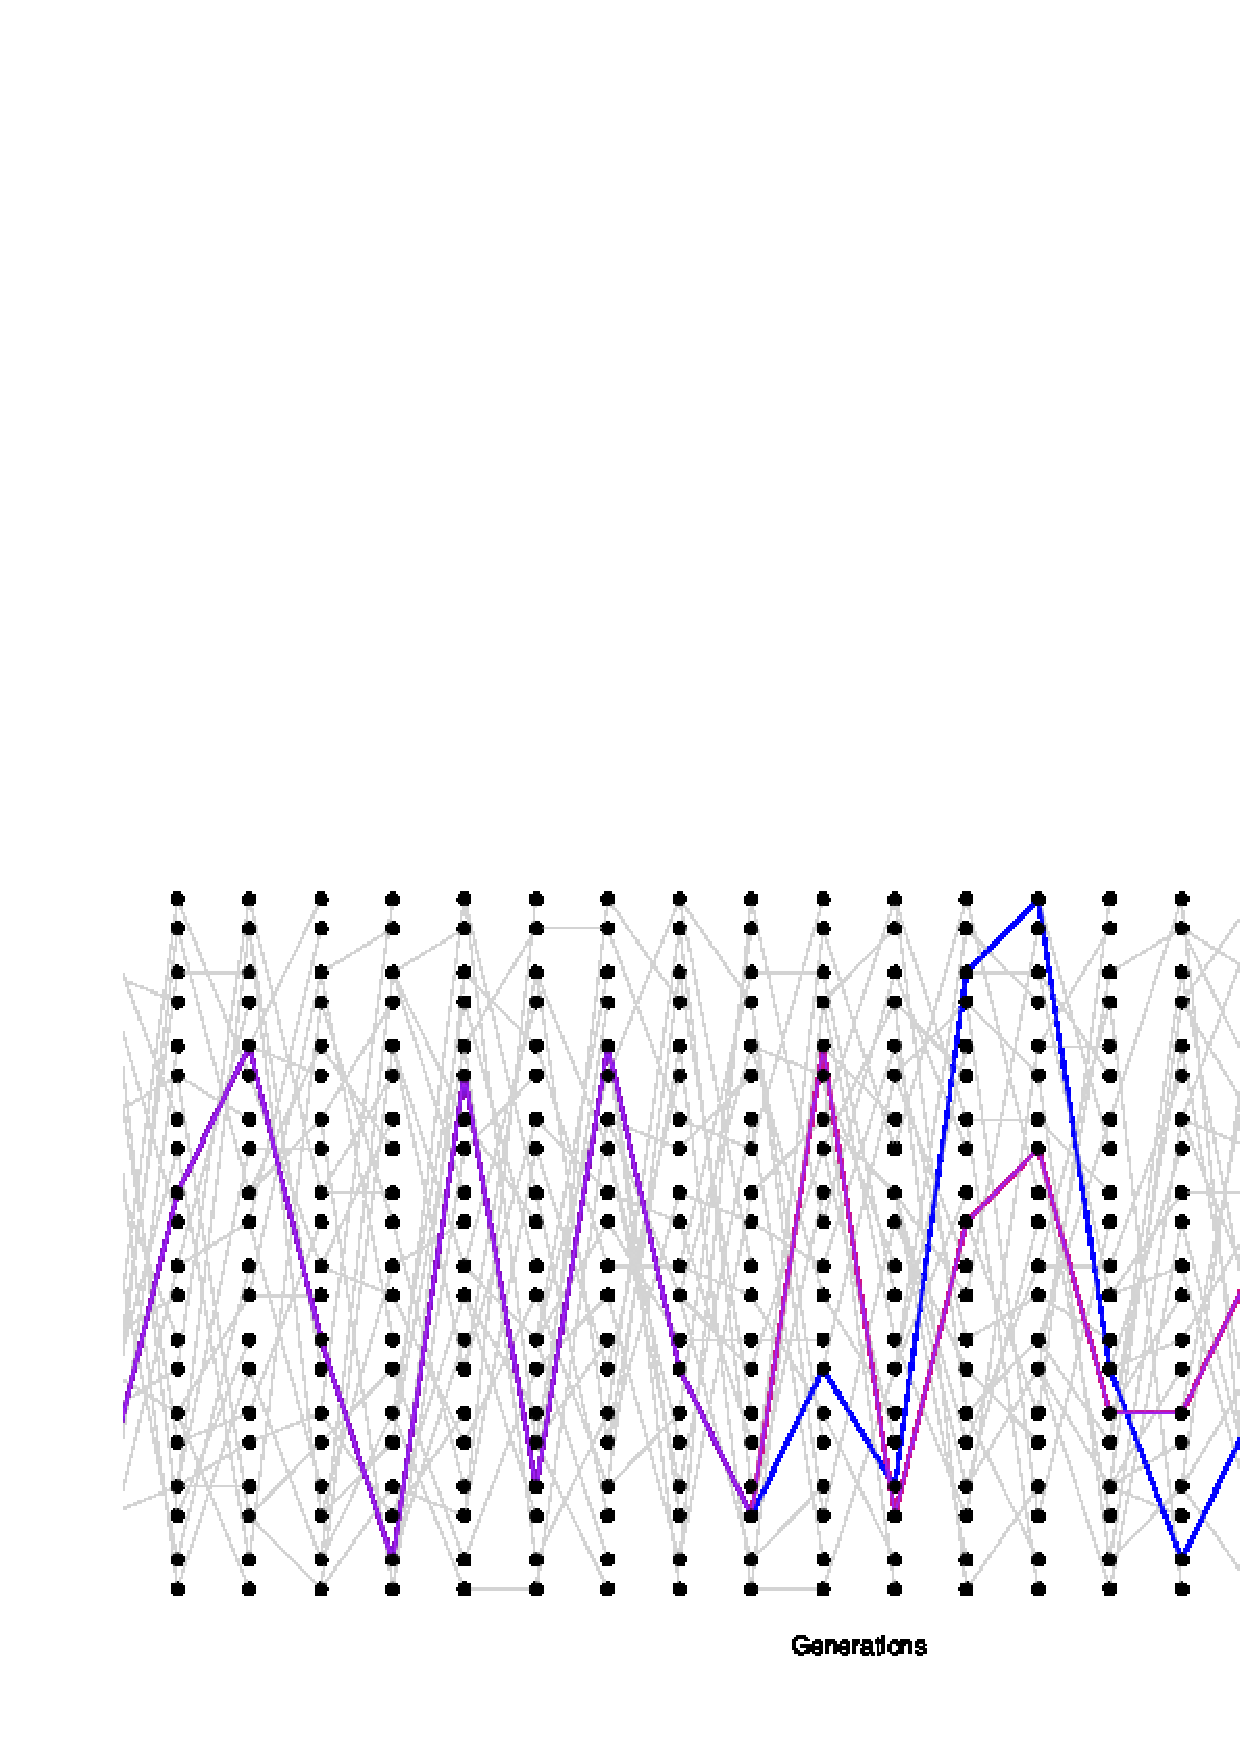
\includegraphics[width = \textwidth]{figures/Coalescent_3.png}
\end{center}
\caption{A simple simulation of the coalescent process for three
  lineages. We track the ancestry of 
  three modern-day alleles, the first pair (blue and purple) coalesce four generations back 
  their are then two independent lineages we are tracking, this pair
  then coalesces twelve generations in the past. Note that different
  random realizations of this process will differ from each other a lot.} \label{fig:Coalescent_simulation_3}
\end{figure}


More generally when we sample $i$ alleles there are ${i \choose
 2}$ pairs, i.e. $i(i-1)/2$ pairs, thus the probability that no pair
of alleles coalesces in the preceding generation is
\begin{equation}
\left(1-\frac{1}{(2N)} \right)^{{i \choose
 2}} \approx \left( 1- \frac{{i \choose
 2}}{2N}\right)
\end{equation}
while the probability of any pair coalescing is $\approx \frac{{i \choose
 2}}{2N}$.\\

We can ignore the possibility of more than pairs of alleles (e.g. tripletons)
simultaneously coalescing at once as terms of $\nicefrac{1}{N^2}$ and higher
can be ignored as they are vanishingly rare. Obviously there are in reasonable
sample sizes there are many more triples (${i \choose 3}$), and higher order
combinations, than pairs (${i \choose 2}$) but if $i \ll N$ then we are safe to
ignore these terms.

When there are $i$ alleles the probability that we wait until the
$t+1$ generation before
any pair of alleles coalesce is
\begin{equation}
 \frac{{i \choose
 2}}{2N}\left( 1- \frac{{i \choose
 2}}{2N}\right)^{t} \approx  \frac{{i \choose
 2}}{2N} \exp \left( - \frac{{i \choose
 2}}{2N} t \right)
\end{equation}
thus the waiting time $T_i$ to the first coalescent event in a sample
of $i$ alleles is exponentially distributed with rate $\frac{{i \choose
2}}{2N}$, i.e. $T_i \sim \text{Exp}\left(\nicefrac{{i \choose
 2}}{2N} \right)$. The mean waiting time till any of pair within our
 sample to coalesce is $\nicefrac{2N}{{i \choose
 2}}$.\\

When a pair of alleles first find a common ancestral allele some
number of generations back further into the past we only have to keep
track of that common ancestral allele for the pair. Thus when a pair
of alleles in our sample of $i$ alleles coalesce, we then switch to
having to follow $i-1$ alleles back. Then when a pair of these $i-1$
alleles coalesce, we then have to follow $i-2$ alleles back. This
process continues until we coalesce back to a sample of two, and from
there to a single most recent common ancestor (MRCA).\\


To simulate a coalescent genealogy at a locus for a sample of $n$ alleles we therefore simply follow this
algorithm
\begin{enumerate}
\item Set $i=n$.
\item We simulate a random variable to be the time $t_i$ to the next coalescent event from $t_i \sim
  \text{Exp}\left(\nicefrac{{i \choose
 2}}{2N} \right)$
\item Choose a pair of alleles to coalesce at random from all possible
 pairs.
\item Set $i=i-1$
\item Continue looping of steps 1-3 until $i=1$ i.e. the most recent
 common ancestor of the sample is found.
\end{enumerate}
by following this algorithm we are generating realizations of the
genealogy of our sample. \\

We will first consider the time to the most recent common ancestor of
the entire sample ($T_{MRCA}$). This is
\begin{equation}
T_{MRCA} = \sum_{i=n}^2 T_i
\end{equation}
generations back. As our coalescent times for different $i$ are independent, the expected time to the most recent common ancestor
is
\begin{equation}
\E(T_{MRCA}) = \sum_{i=n}^2 \E(T_i) = \sum_{i=n}^2  2N/{i \choose
 2}
\end{equation}
using the fact that $\frac{1}{i(i-1)}=\frac{1}{i-1} - \frac{1}{i}$ with a bit of
rearrangement we can rewrite this is
\begin{equation}
\E(T_{MRCA}) = 4N\left(1- \frac{1}{n} \right)
\end{equation}
so the average $T_{MRCA}$ scales linearly with population
size. Interestingly, as we move to larger and larger samples (i.e. $n \gg 1$) the average
time to the most recent common ancestor is converging on $4N$. What's
happening here is that in large samples our lineages typically coalesce rapidly
at the start and very soon coalesce down to a much smaller number of
lineages.   \\

% TODO
Above we argued that a mutation only becomes a fixed difference if it is lucky
enough to be the ancestor of the entire population. As we saw above this occurs
with probability $\nicefrac{1}{(2N)}$. How long does is take on average for
such an allele to fix within our population? We've just seen that it takes $4N$
generations for a large sample of alleles to all trace their ancestry back to a
single most recent common ancestor. Thus it must take roughly $4N$ generations
for a neutral allele present in a single copy within the population to the
ancestor of all alleles within our population. This argument can be made more
precise, but in general we would still find that it takes $\approx 4N$
generations for a neutral allele to go from its introduction to fixation with
the population.   \\


%%point about the fixation time of a neutral allele

\paragraph{The total amount of time in a genealogy}

Mutations fall on lineages of the coalescent genealogy. These mutations affect all
descendants of this lineage, and under the infinitely-many-sites assumption,
create a new segregating site for each new mutation. The mutation process is a
\emph{Poisson process}, and the longer a particular lineage branch, the more
mutations that can accumulate on it. The total number of segregating sites in
the genealogy is thus a function of the \emph{total} amount of time in the
genealogy of the sample, or the sum of all the genealogy branch lengths,
$T_{tot}$. Since our coalescent genealogies are bifurcating (only two lineages
coalesce at once), our total amount of time in the genealogy is:

\begin{equation}
T_{tot} = \sum_{i=n}^2 iT_i
\end{equation}
as when there are $i$ lineages each contributes a time $T_i$ to the
total time. Taking the expectation of the total time in the genealogy
\begin{equation}
\E(T_{tot}) = \sum_{i=n}^2 i \frac{2N}{{i \choose
 2} } = \sum_{i=n}^2 \frac{4N}{i -1} =\sum_{i=n-1}^1 \frac{4N}{i}
\end{equation}
so our expected total amount of time in the genealogy scales linearly
with our population size. Our expected total amount of time is also
increasing with sample size but is doing so very slowly. To see this
more carefully we can see that for large $n$
\begin{equation}
\E(T_{tot}) = \sum_{i=n-1}^1 \frac{4N}{i} \approx 4N \int_1^n \frac{1}{i} di
= 4N \log(n-1)
\end{equation}
here we are approximating our sum by an integral, which will work for
large $n$. So our expected total amount of time in the genealogy
is growing with $n$ but it is doing so very slowly. This again follows
from the fact that in large samples the initial coalescence usually
happens very rapidly, so that extra samples adds little to the total
amount of time in the tree. \\

We saw above that the number of mutational differences between a pair
of alleles that coalescence $T_2$ generations ago was Poisson with a
mean of $2 \mu T_2$. A mutation that occurs on any branch of our
genealogy will cause a segregating polymorphism in the sample
(making our infinitely-many-sites assumption). Thus if the total time
in the genealogy is $T_{tot}$ there is $T_{tot}$
generations for mutations. So the total number of mutations
segregating in our sample ($S$) is Poisson with mean $\mu T_{tot}$. Thus the
expected number of segregting  in history a sample of size $n$ is
\begin{equation}
\E(S) = \mu \E(T_{tot}) = \sum_{i=n-1}^1 \frac{4N\mu }{i} = \theta
\sum_{i=n-1}^1 \frac{1}{i}
\end{equation}
Thus we can use this formula to derive another estimate of the
population scaled mutation rate, by setting our observed number of
segregating sites in a sample ($S$) equal to this expectation. We'll call this estimator $\widehat{\theta}_W$
\begin{equation}
\widehat{\theta}_W =\frac{ S}{\sum_{i=n-1}^1 \frac{1}{i}}  
\end{equation}
this estimator was devised by Watterson, hence the $W$.


\subsection{The fixation of neutral alleles}
It is very unlikely that a rare neutral allele accidentally drifts up
to fixation, it is much more likely that such an allele is eventually
lost from the population. However, there is a large and constant influx of
rare alleles into the population due to mutation, so even if it is very
unlikely that an individual allele fixes within the population, some
neutral alleles will fix.  \\

%We'll first consider the probability that a neutral allele fixes
%within the population, starting from it just enters a diploid
%population as a newly mutated allele at frequency $1/(2N)$.

%so for an allele to be fixed in the population it
%must have been that allele


\paragraph{Probability of the eventual fixation of a neutral allele.} An allele which reaches fixation within a population, is an ancestor to
the entire population. In a particular generation there can be only single
allele that all other alleles at the locus in  later generation can claim as an
ancestor. As at a neutral locus all of our alleles are exchangeable, as
they have no effect on the number of descendents an individual
leaves, so any allele is equally likely to be the ancestor of the
entire population.  In a diploid population size of size $N$, there are $2N$
alleles all of which are equally likely to be the ancestor of the
entire population at some later time point. So if our allele is present in a single copy, the chance that
is the ancestor to the entire population in some future generation is
$1/(2N)$, i.e. the chance our neutral allele is eventually fixed is
$1/(2N)$. See Figure \ref{fig:subs_simulation}, our orange allele in
the first generation is one of 10 differently coloured alleles, 
and so has a $1/10$ chance of being  the ancestor of the entire
population at some later time point (as it is by the 9th generation).\\

More generally if our neutral allele is present in $i$ copies in the
population, of $2N$ alleles, the probability that this allele is fixed
is $i/(2N)$. I.e. the probability that a neutral allele is eventually
fixed is simply given by its frequency ($p$) in the population.
We can also derive this result by letting $Ns \rightarrow
0$ in eqn. \eqref{eqn:prob_fixed}.

\begin{figure}
\begin{center}
  \includegraphics[width = \textwidth]{figures/Substitution_sim.png}
\end{center}
\caption{Each allele initially present in a small diploid population is
  given a different colour so we can track their descendants over
  time. By the 9th generation all of the alleles present in the
  population can trace their ancestry back to the orange allele.} \label{fig:subs_simulation}
\end{figure}

\paragraph{Rate of substitution of neutral alleles.}

A substitution between populations that do not exchange gene flow is
simply a fixation event within one population. The rate of
substitution is therefore the rate at which new alleles fix in the
population, so that the long-term substitution rate is the rate at
which mutations arise that will eventually become fixed within our population.\\

Assume that there are two classes of mutational changes that can occur with a
region, highly deleterious mutations and neutral mutations. A fraction
$C$ of all mutational changes are highly deleterious, and can not
possibly contribute to substitution nor polymorphism (i.e. $Ns \gg 1$).
While a fraction $1-C$ are neutral. If our mutation rate is $\mu$ per
transmitted allele per generation, then a total of $2N \mu (1-C)$
neutral mutations enter our population each generation.\\

Each of these neutral mutations has a $1/(2N)$ probability chance of
eventually becoming fixed in the population. Therefore, the rate at
which neutral mutations arise that eventually become fixed within our
population is  
\begin{equation}
2N\mu(1-C)\frac{1}{2N} = \mu(1-C)
\end{equation}
thus the rate of substitution under a model where newly arising alleles are either
highly deleterious or neutral, is simply given by the mutation rate
towards neutral alleles, i.e. $\mu(1-C)$.\\

Consider a pair of species have diverged for $T$ generations, i.e. orthologous sequences shared between the species last shared a common ancestor $T$ generations ago. If they have maintained a constant $\mu$ over that time, will have accumulated an average of
\begin{equation}
2\mu(1-C)T
\end{equation}
neutral substitutions. This assumes that $T$ is a lot longer than the time it
takes to fix a neutral allele, such that the total number of 
alleles introduced into the population that will eventually fix is the
total number of substitutions. We'll see below that a neutral allele
takes on average $4N$ generations to fix from its introduction into
the population.\\

This is a really pretty result as the population size has completely
canceled out of the neutral substitution rate. However, there is
another way to see this in a more straightward way. If I look at a
sequence in me compared to say a particular chimp, I'm looking at the mutations
that have occurred in both of our germlines since they parted ways $T$
generations ago. Since neutral alleles do not alter the probability
of their transmission to the next generation, we are simply looking at
the mutations that have occurred in $2T$ generations worth of
transmissions. Thus the average number of neutral mutational
differences separating our pair of species is simply $2\mu (1-C) T$.\\

\begin{question}
For this, and the next question, assume that humans and chimp diverged
around 5.5$\times 10^6$ years, a generation time ~20 years, that the speciation occurred instantaneously in allopatry with no subsequent gene flow, and the ancestral effective population size of the human and chimp common ancestor population was 10,000 individuals.\\
Nachman and Crowell sequenced 12 pseudogenes in human and chimp found substitutions at 1.3\% of sites. \\
{\bf A) } What can you say about the mutation rate per site per generation at these genes, and how does it compare to other estimates of human mutation rate?\\
{\bf B)} All of the pseudogenes they sequenced are on the autosomes. What
would you prediction be for pseudogenes on the X and Y chromosomes,
given that there are fewer rounds of replication in the female
germline than in the male germline.
\end{question}




\subsection{Neutral diversity and population structure}
%%this section was moved from the coalescent chapter
Upto now we have assumed that our alleles that we have modelled in the
coalescent setting are drawn from a randomly mating population such
that any pair of lineages is equally likely to coalesce with each
other. However, when there is population structure this assumption is
violated. \\

We have previously written the measure of population structure
$\fst$ as
\begin{equation}
\fst = \frac{H_T-H_S}{H_T}
\end{equation}
where $H_S$ is the probability that two alleles sampled at random from a
subpopulation differ, and $H_T$ is the probability that two alleles
sampled at random from the total population differ. 

\paragraph{A simple population split model}
Imagine a population of constant size of $N_e$ diploid individuals that
$\tau$ generations in the past split into two daughter populations (sub-populations)
each of size $N_e$ individuals, who do not subsequently exchange
migrants. In the current day we sample an equal number of alleles
from both subpopulations.

Consider a pair of alleles sampled within one of our
sub-populations, they have experienced a population of size $N_e$
and so the probability that they differ is $H_S = \theta/(1+\theta)$
(where $\theta=4N_e\mu$).
The heterozygosity in our total population is a little more tricky to
calculate. Assuming that we equally sample both sub-populations, when we draw two alleles from our total
sample, $50\%$ of the time they are drawn from the same
subpopulation and $50\%$ of the time they are drawn from different
subpopulations. Therefore, our total heterozygosity is given by
\begin{equation}
H_T = \half H_S + \half H_B
\end{equation}
where $H_B$ is the probability that a pair of alleles drawn from our
two different sub-populations differ from each other. Our pair of
alleles can not find a common ancestor with each other for at least $\tau$
generations into he past as they are in distinct populations (not
connected by migration). The probability that one or other of them
mutates in this time is $1-(1-\mu)^{2T}$. With probability
$(1-\mu)^{2T} $ neither of our alleles mutate in the $T$ generations
back in time before they find themselves back in the combined ancestral 
population. Conditional on failing to mutating before the combined ancestral
population, the probability that they do manage to mutate before
coalescing in that population of size $N_e$ is
$\theta/(\theta+1)$. Putting these components together
\begin{equation}
H_B = \left( 1-(1-\mu)^{2T} \right) + (1-\mu)^{2T}
  \frac{\theta}{\theta+1} 
\end{equation}
We can plug this into our expression for $H_T$, and then that in turn
into $\fst$.

\begin{figure}
\begin{center}
\includegraphics[width= 0.8 \textwidth]{figures/drift_split.png}
\end{center}
\caption{Change in allele frequencies following a population split.} \label{fig:drift_split}  
\end{figure} 

To understand this better we can make a simple
approximation based on our mutation rate being very low, such that
$N_e \mu \ll 1$ ao $H_S \approx
4N_e\mu$, and that $\mu \ll 1$ and $\mu T \ll 1$. Assuming this, then  
\begin{equation}
H_B \approx 2 \mu T + 4N_e\mu. 
\end{equation}
So that 
\begin{equation}
\fst \approx \frac{ \mu T}{\mu T +  4N_e\mu }  %= \frac{ T}{ T +  4N_e }
\end{equation}
note that $\mu$ cancels out of this. In this simple toy model $\fst$
is increasing because the amount of between population diversity 
increases with the divergence time of the two populations (initially
linearly with $T$). It does so at a rate
give by $T/(4N_e)$ so that differentiation will be higher
between populations separated by long divergence times or with small
effective population sizes.

\begin{question}
The gorilla lineage split from the human-chimp lineage $\sim$7 million years ago. Let’s assume that this speciation event occurred instantaneously in allopatry with no subsequent gene flow. \\
{\bf A)}	What is the probability of that Gorilla is not an outgroup to human and chimp at a single locus?\\
{\bf B)}	It has been estimated that the Gorilla lineage is not an outgroup at around ~30\% of autosomal loci. What effective population size would you need to assume to explain this observation? Is that only plausible explanation?\\
{\bf C)}	The Gorilla lineage is an outgroup for large portions of the X chromosome, what is a plausible explanation for this finding?
\end{question}

\paragraph{A simple model of migration between an island and the mainland.}
We can also use the coalescent to think about patterns of
differentiation under a simple model of migration drift
equilibrium. Lets consider a small island population that is relatively isolated
from a large mainland population, and that both of these populations
are constant in size. We'll assume that the expected heterozygosity
for a pair of alleles sampled on the mainland is $H_M$.

Our island has a population size
$N_{I}$ that is very small compared to our mainland population.
Each generation some low fraction $m$ of our individuals on the
island have migrant parents from the mainland the generation
before. Our island may also send migrants back to the mainland, but
these are a drop in the ocean compared to the large population size on
the mainland and their effect can be ignored. 


If we sample an allele on the island back and trace its ancestral
lineage backward in time, each generation our ancestral allele have a low
probability $m$ of being descended from the mainland in the proceeding
generation (if we go far enough the allele eventually has to be
descended from an allele on the mainland). The probability that a pair of alleles sampled on the
island are descended from a shared recent common ancestral allele on the island, is the
probability that our pair of alleles coalesce before either lineage
migrates. For example, the probability that our pair of alleles
coalesce $t+1$ generations back is 
\begin{equation}
\frac{1}{2N_I}(1-m)^{2(t+1)} \left(1-\frac{1}{2N_I} \right)^{t} \approx
\frac{1}{2N_I} \exp\left( -t\left (\frac{1}{2N_I} + 2m\right) \right),
\end{equation}
with the approximation following from assuming that $m \ll 1$ \& $1/(2N_I)
\ll 1$ (note that this is very similar to our derivation of
heterozygosity above). The probability that our alleles coalescence before either one
of them migrates off the island, irrespective of the time, is
\begin{equation}
\int_0^{\infty} \frac{1}{2N_I} \exp\left( -t\left (\frac{1}{2N_I} +
    2m\right) \right) dt = \frac{1/(2N_I) }{1/(2N_I) +
    2m}.
\end{equation}

Lets assume that the mutation rate is very low such as it is very
unlikely that the pair of alleles mutate before they coalesce on the
island. Therefore, the only way that the alleles can be different from
each other is if one or other of them migrates to the mainland, which
happens with probability  
\begin{equation}
1 - \frac{1/(2N_I) }{1/(2N_I) + 2m}
\end{equation}
Conditional on one or other of our alleles migrating to the mainland,
both of our alleles represent independent draws from the mainland and
so differ from each other with probability $H_M$. Therefore, the level of
heterozygosity on the island is given by
\begin{equation}
H_I = (1 - \frac{1/(2N_I) }{1/(2N_I) + 2m})H_M
\end{equation}
So the reduction of heterozygosity on the island compared to the
mainland is
\begin{equation}
F_{IM} = 1- \frac{H_I}{H_M} = \frac{ 1/(2N_I) }{1/(2N_I) + 2m} = \frac{ 1 }{1 + 4N_Im}.
\end{equation}
The level of inbreeding on the island compared to the mainland will
be high in the migration rate is low and the effective population size
of the island is low, as allele frequencies on the island are drifting
and diversity is not being replenished on the island by migration. The
key parameter here is the number individuals on the island replaced by
immigrants from the mainland each generation ($N_I m$).

We have framed this as being about the reduction in genetic diversity on the
island compared to the mainland. However, if we consider collecting a
individuals on the island and mainland in proportion to population
sizes the total level of heterozygosity would be $H_T=H_M$, as samples
from our mainland would greatly outnumber those from our
island. Therefore, considering our island our sub-population we have
derived another simple model of $F_{ST}$ .

\begin{question}
You are investigating a small river population of sticklebacks, which receives infrequent migrants from a very large marine population. At a set of (putativelyneutral biallelic markers the freshwater population has frequencies:\\
0.2, 0.7, 0.8\\
at the same markers the marine population has frequencies:\\
0.4, 0.5 and 0.7.\\
 From studying patterns of heterozygosity at a large collection of markers, you have estimated the long term effective size of your freshwater population is 2000 individuals.\\
What is your estimate of the migration rate from the marine
populations into the river?
\end{question}
\newpage

